\documentclass{article}
\usepackage{tikz}
\usetikzlibrary{positioning}
\usetikzlibrary{shapes.geometric}
\usetikzlibrary{shapes.symbols} \usetikzlibrary{shadows}
\usetikzlibrary{arrows}

\pagestyle{empty}

\begin{document}

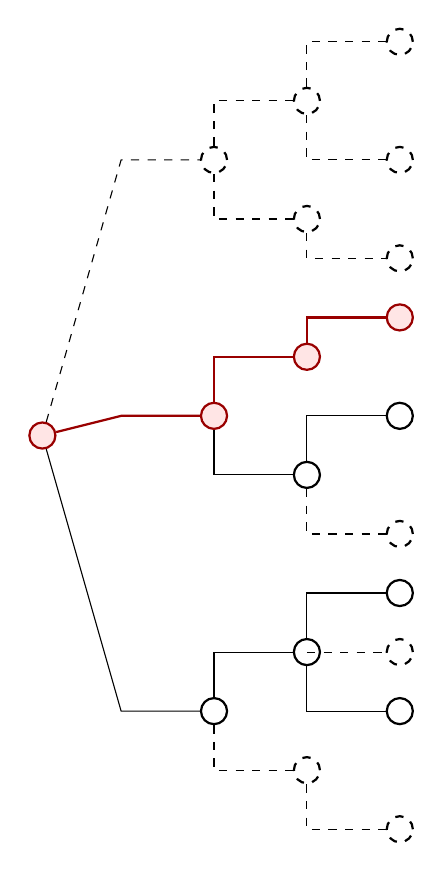
\begin{tikzpicture}
[node/.style={shape=rectangle,draw,thick,right},
 node/.style={shape=ellipse,draw,thick,right},
 selected/.style={draw=red!60!black},
 seledge/.style={selected,thick},
 selnode/.style={red!60!black,selected,fill=red!10!white}]

\draw (0,0) node (root) [node,selnode] {};

\draw [dashed] (root) -- ++(1.0,3.5) -- ++(1.0, 0)
	node (s1) [node] {};
\draw [dashed] (s1) -- ++(0, 0.75) -- ++(1.0, 0)
	node (s11) [node] {};
\draw [dashed] (s1) -- ++(0, -0.75) -- ++(1.0, 0)
	node (s12) [node] {};
\draw [dashed] (s11) -- ++(0, 0.75) -- ++(1.0, 0)
	node (s111) [node] {};
\draw [dashed] (s11) -- ++(0, -0.75) -- ++(1.0, 0)
	node (s112) [node] {};
\draw [dashed] (s12) -- ++(0, -0.5) -- ++(1.0, 0)
	node (s121) [node] {};

\draw [seledge] (root) -- ++(1.0,0.25) -- ++(1.0, 0)
	node (s2) [node,selnode] {};
\draw [seledge] (s2) -- ++(0, 0.75) -- ++(1.0, 0)
	node (s21) [node,selnode] {};
\draw (s2) -- ++(0, -0.75) -- ++(1.0, 0)
	node (s22) [node] {};
\draw [seledge] (s21) -- ++(0, +0.5) -- ++(1.0, 0)
	node (s211) [node,selnode] {};
\draw (s22) -- ++(0, 0.75) -- ++(1.0, 0)
	node (s221) [node] {};
\draw [dashed] (s22) -- ++(0, -0.75) -- ++(1.0, 0)
	node (s222) [node] {};

\draw (root) -- ++(1.0,-3.5) -- ++(1.0, 0)
	node (s3) [node] {};
\draw (s3) -- ++(0, 0.75) -- ++(1.0, 0)
	node (s31) [node] {};
\draw [dashed] (s3) -- ++(0, -0.75) -- ++(1.0, 0)
	node (s32) [node] {};
\draw (s31) -- ++(0, 0.75) -- ++(1.0, 0)
	node (s311) [node] {};
\draw [dashed] (s31) -- ++(0, -0.0) -- ++(1.0, 0)
	node (s312) [node] {};
\draw  (s31) -- ++(0, -0.75) -- ++(1.0, 0)
	node (s313) [node] {};
\draw  [dashed] (s32) -- ++(0, -0.75) -- ++(1.0, 0)
	node (s311) [node] {};
\end{tikzpicture}
\end{document}
